\section{Simulation and Analysis}
In this section, a vehicle-fluid coupling co-simulation verification platform is established. Based on this platform, three extreme scenarios, including left turn, high-speed single lane change (SLC), and short-distance double lane change (DLC), are simulated and validated.

\vspace{-0.3cm}
\subsection{Simulation Platform Construction}

\begin{figure*}[!hbt]
  \centering
  \subfloat[]{
    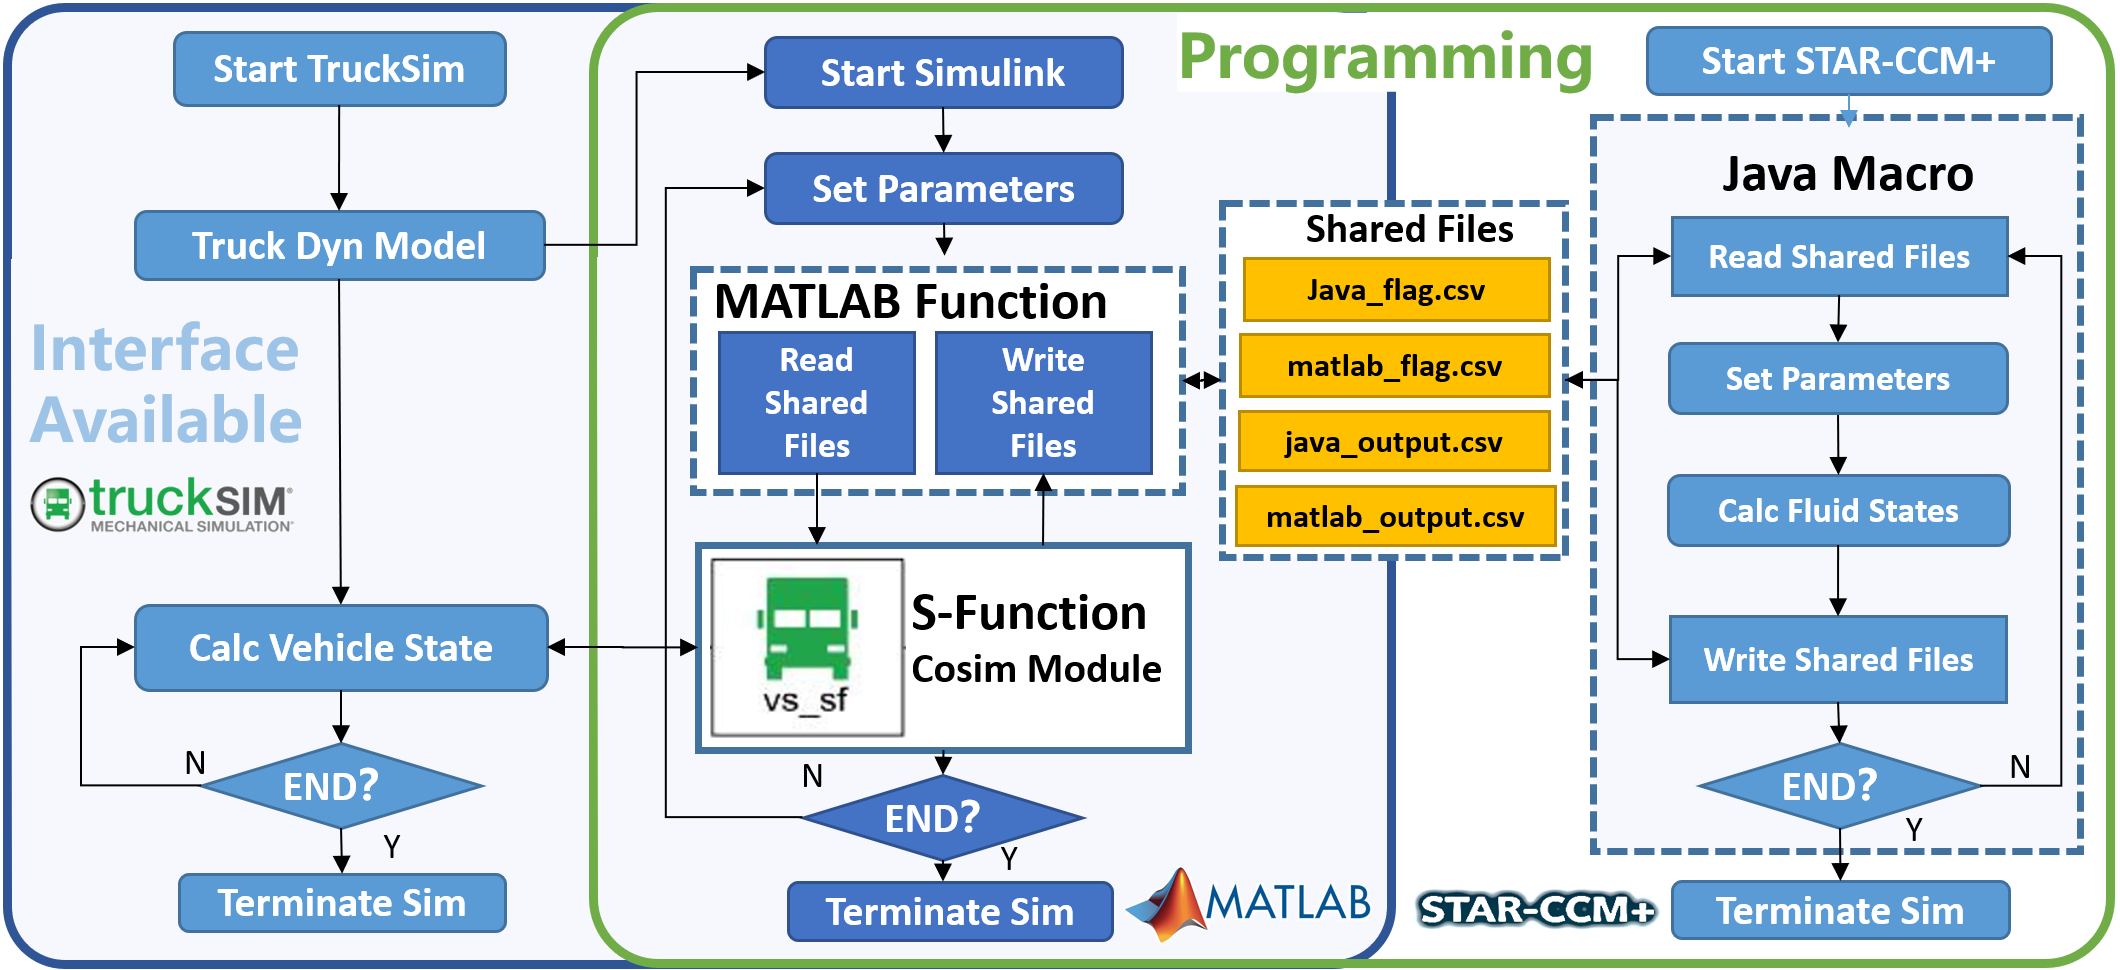
\includegraphics[width=0.55\textwidth]{fig/cosim_platform.png}
    \label{fig:cosim_platform}}
 % \hfill
  \subfloat[]{
    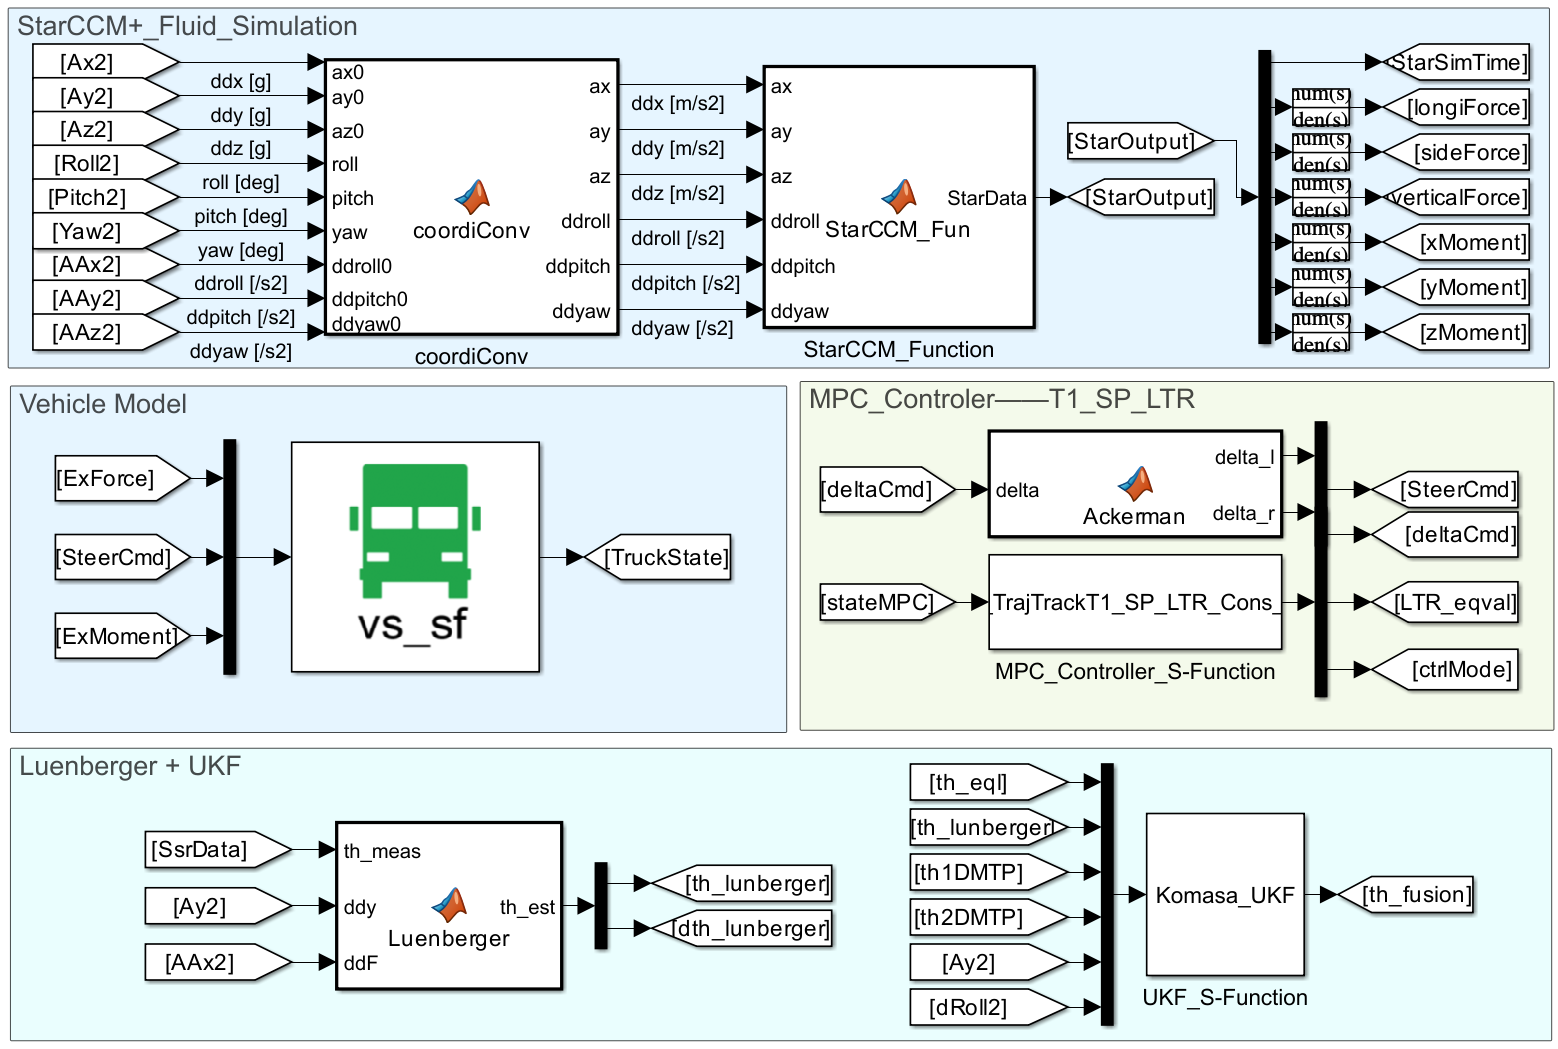
\includegraphics[width=0.37\textwidth]{fig/SimulinkModel.png}
    \label{fig:simulink}} 

  \vspace{-0.5cm}
  \subfloat[]{
    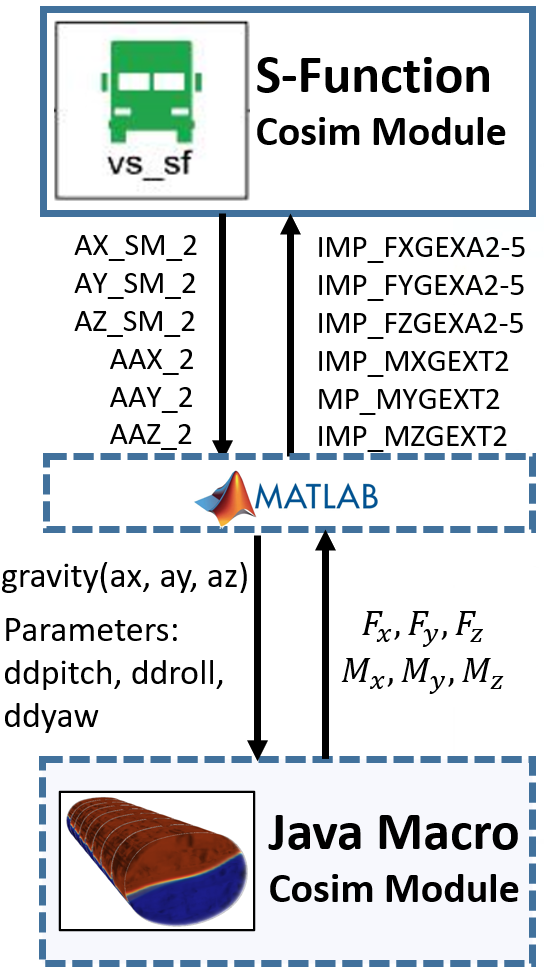
\includegraphics[width=0.14\textwidth]{fig/cosim_variable.png}
    \label{fig:cosim_variable}
  }
  \subfloat[]{
    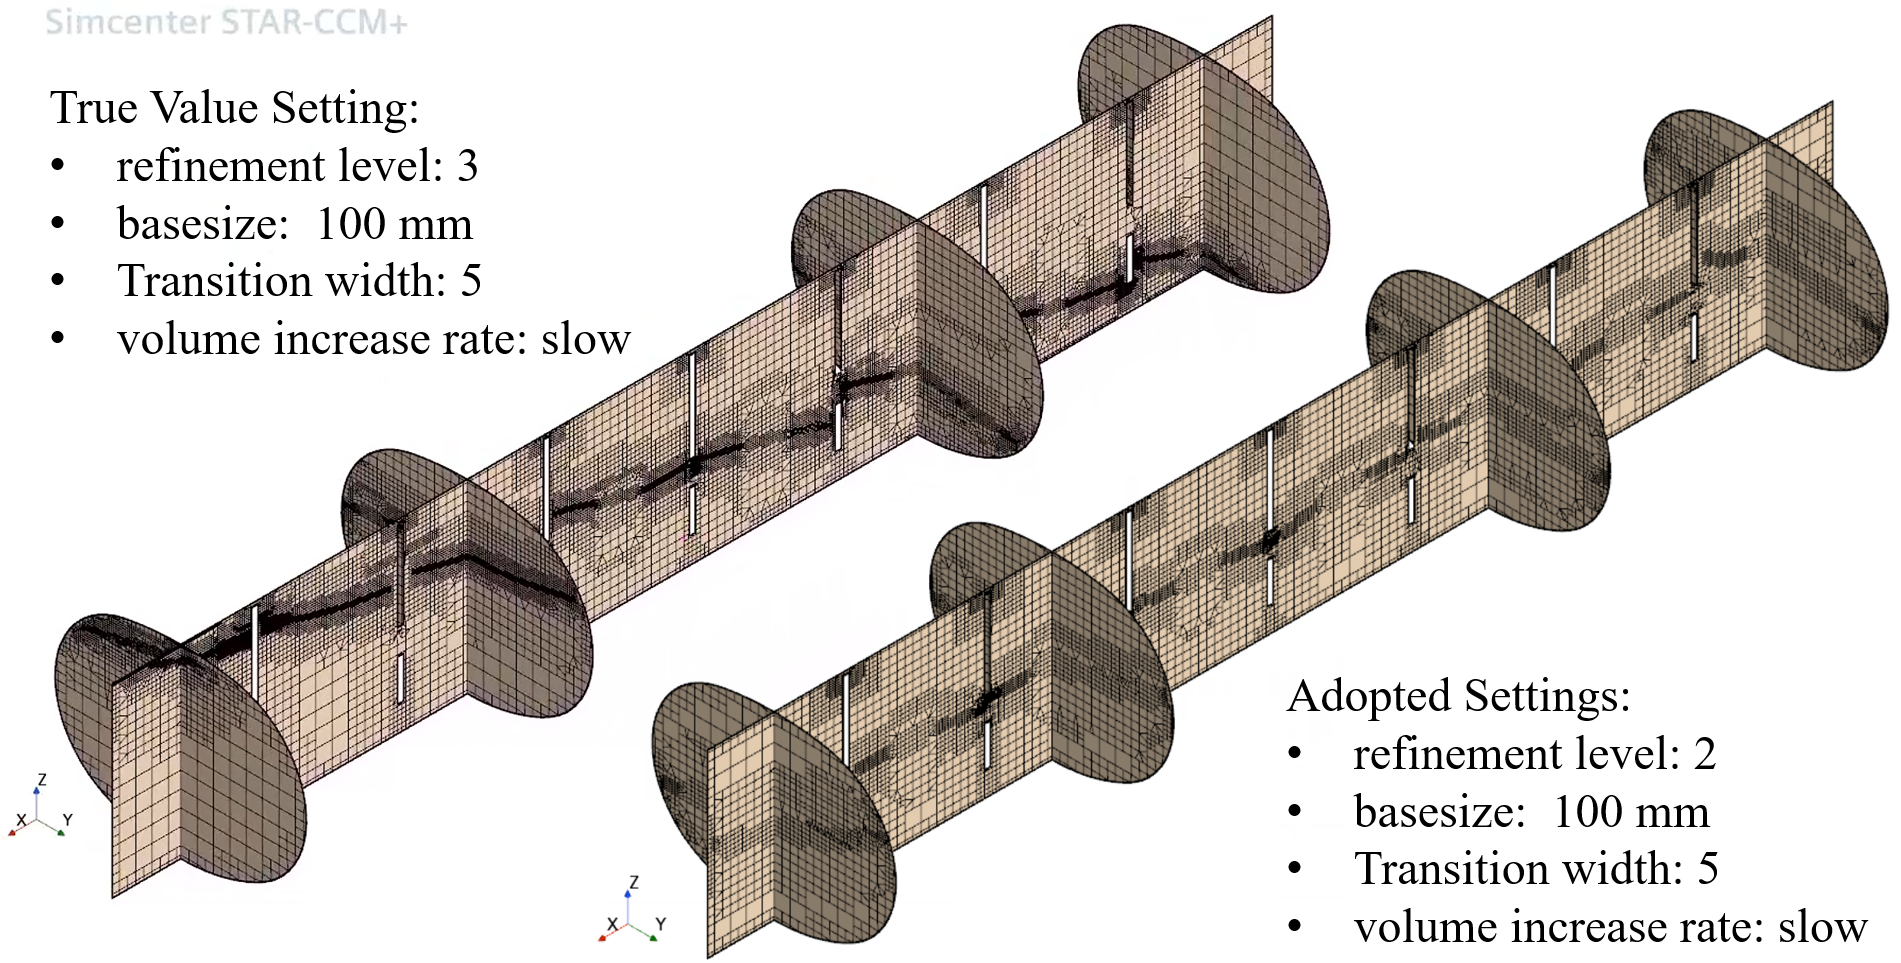
\includegraphics[width=0.5\textwidth]{fig/cosim_grid.png}
    \label{fig:grid}
  }
  \subfloat[]{
    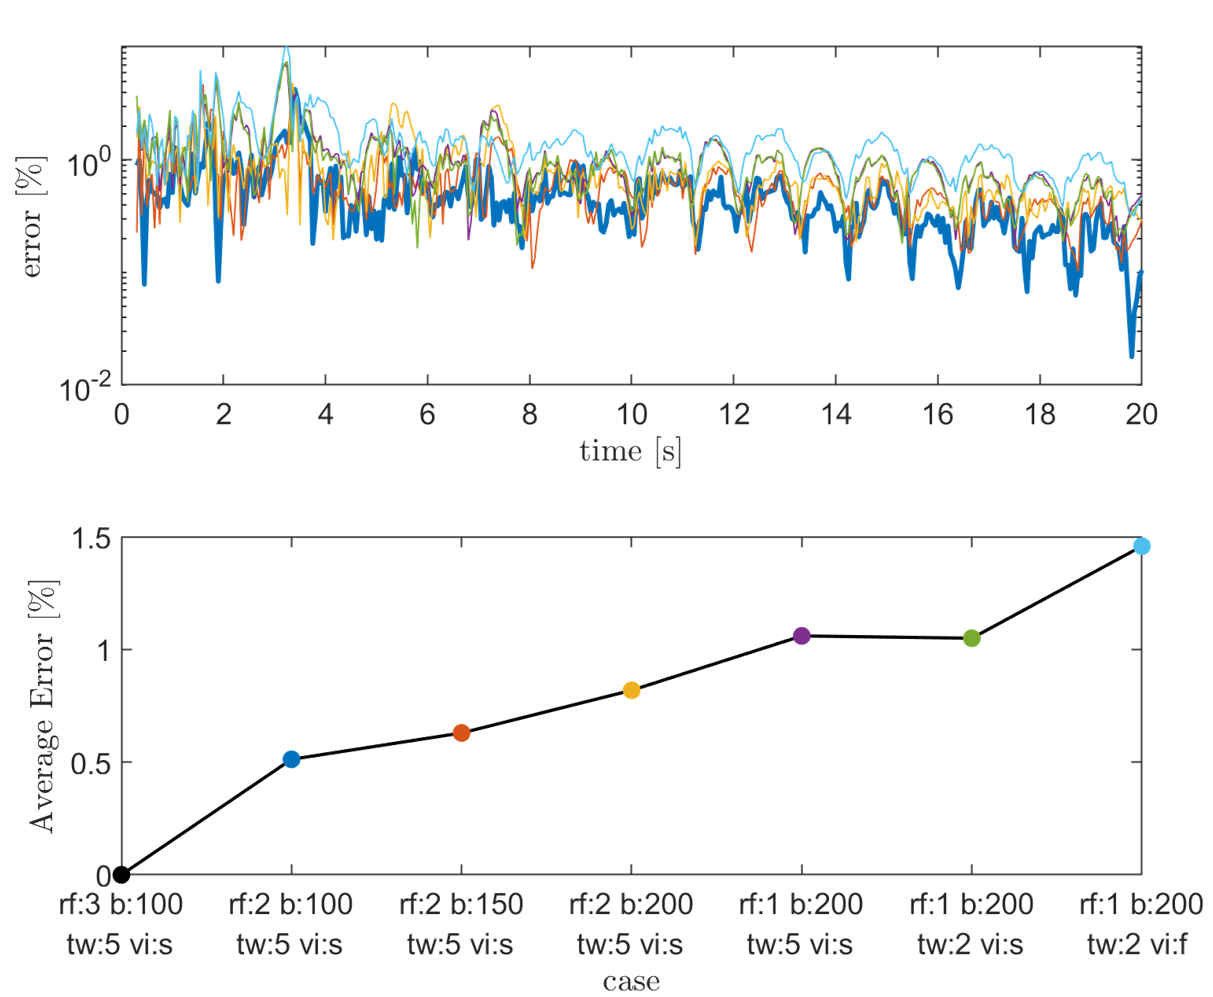
\includegraphics[width=0.3\textwidth]{fig/cosim_grid_sensitivity.png}
    \label{fig:sensitivity}
  }
  
  \caption{Co-simulation platform and grid sensitivity. (a)Logic architecture of co-simulation platform. (b)Co-simulation model constructed in MATLAB/Simulink. (c)Parameter connection of co-simulation platform. (d)Mesh settings for true value and adopted model for co-simulation. (e)Error and time average error of $F_x$, $F_y$, $F_z$, $M_x$, $M_y$, and$M_z$ for grid sensitivity check, where rf is refinement level, b is basesize of mesh, tw is transition width, vi is volume growth rate, s and f are abbreviations for slow and fast, respectively.}
  \label{fig:cosim}
  \vspace{-0.3cm}
\end{figure*}

To better validate the effectiveness of the proposed anti-rollover path tracking control, a vehicle-fluid coupling co-simulation platform, as shown in Fig. \ref{fig:cosim}, was constructed. The fluid was accurately simulated using the finite volume method (FVM) based computational fluid dynamics (CFD) method. MATLAB Function and Java macros are designed to enable data exchange between Simulink and StarCCM+. Two flag files and two data exchange files are created to facilitate parameter-level interaction, as illustrated in Fig. \ref{fig:cosim_platform} In each time step, as in Fig. \ref{fig:cosim_variable}, TruckSim provided the acceleration and angular acceleration of the sprung mass of the trailer, which are applied to the fluid in StarCCM+ through changing components of the gravity model and user-defined volume forces (see Table.\ref{tab:sim_settings}, UDF). Meanwhile, StarCCM+ provides the three-dimensional forces and moments exerted on the tank by fluid, which are applied to the semi-trailer in TruckSim. This co-simulation approach enables real-time (in simulation) interaction and mutual influence between vehicle dynamics and CFD. A simulation model, as shown in Fig. \ref{fig:simulink}, is built in Simulink.

To ensure accurate and efficient simulations, a grid sensitivity analysis is conducted. Unit acceleration and angular acceleration excitations are applied to the liquid. The simulation results under specific settings (Fig. \ref{fig:grid}, left) are considered as the reference. Six alternative settings are compared, and their relative errors are shown in Fig. \ref{fig:sensitivity}. The selected settings (Fig. \ref{fig:grid} right, bold blue curve in Fig. \ref{fig:sensitivity}) achieve an average relative error within 1\% and a peak error below 4\%. For more details on the settings, refer to Table \ref{tab:sim_settings}. Liquid sloshing observation in simulation is done with DMTP and Unscented Kalman Filter; details please refer to \cite{KomasaMutiDOF}.

The computer for co-simulation uses 13th Gen Intel$^\circledR$ Core$^{\text{TM}}$  i9-13900HX 2.20GHz with 32GB RAM.

\vspace{-0.5cm}
\begin{table}[!htbp]
  \centering
  \caption{Co-Simulation Settings}
  \vspace{-0.2cm}
  \label{tab:sim_settings}
  \begin{tabularx}{0.45\textwidth}{@{}lX@{}}
    \toprule
    \textbf{Item} & \textbf{Settings} \\
    \midrule
    Software Config. & Matlab R2023a, StarCCM+ 16.06.008-R8, TruckSim 2019.0\\
    Time step & TruckSim:0.001[s], StarCCM+:adaptive(1e-4[s]-0.005[s]), Data exchange:0.005[s] \\
    Dimension & Three-dimensional \\
    Euler phases & C8H17(Gasoline) \& Air, with filling rate 50\% \\
    Flow regime & Segregated flow \\
    Turbulent model & Realizable $k-\epsilon$ two-layer model\\
    Adaptive time step & Time provider:Free surface CFL condition \\
    Volume mesh & Adaptive free surface mesh refinement level: 2, basesize: 100[mm], transition width: 5, volume growh rate: slow\\
    Gravity & Yes, modified each time step by Java Macro \\
    UDF(in code) & 
    \begin{scriptsize}\${Density}*[(\$\${Position}[2]*\${ddpitch}+\$\${Position}[1]*\${ddyaw}), (\$\${Position}[2]*\${ddroll}+\$\${Position}[0]*\${ddyaw}), (\$\${Position}[0]*\${ddpitch}+\$\${Position}[1]*\${ddroll})]\end{scriptsize}\\
    MPC settings & controller frequency: 20 $Hz$, predictive horizon $N_p=40$, control steps $N_c = 3$, and constraint steps $N_r = 15$\\
    Vehicle Model & 3A Sleeper Tractor with 2A Flatbed Trailer (default nonlinear parameters)\\
    \bottomrule
  \end{tabularx}
  \vspace{-0.3cm}
\end{table}








\subsection{Simulation in Different Scenarios}

In this section, the anti-rollover control is validated in 3 typical dangerous conditions, and is compared with TruckSim default preview tracking(PT) and PT with LQR based differential braking \cite{Reviewer2_SunWencai2022,ZhaoWeiqiang2019}.

\subsubsection{left turning scenario}

\begin{figure}[!bt]
  \centering
    \vspace{-0.3cm}
    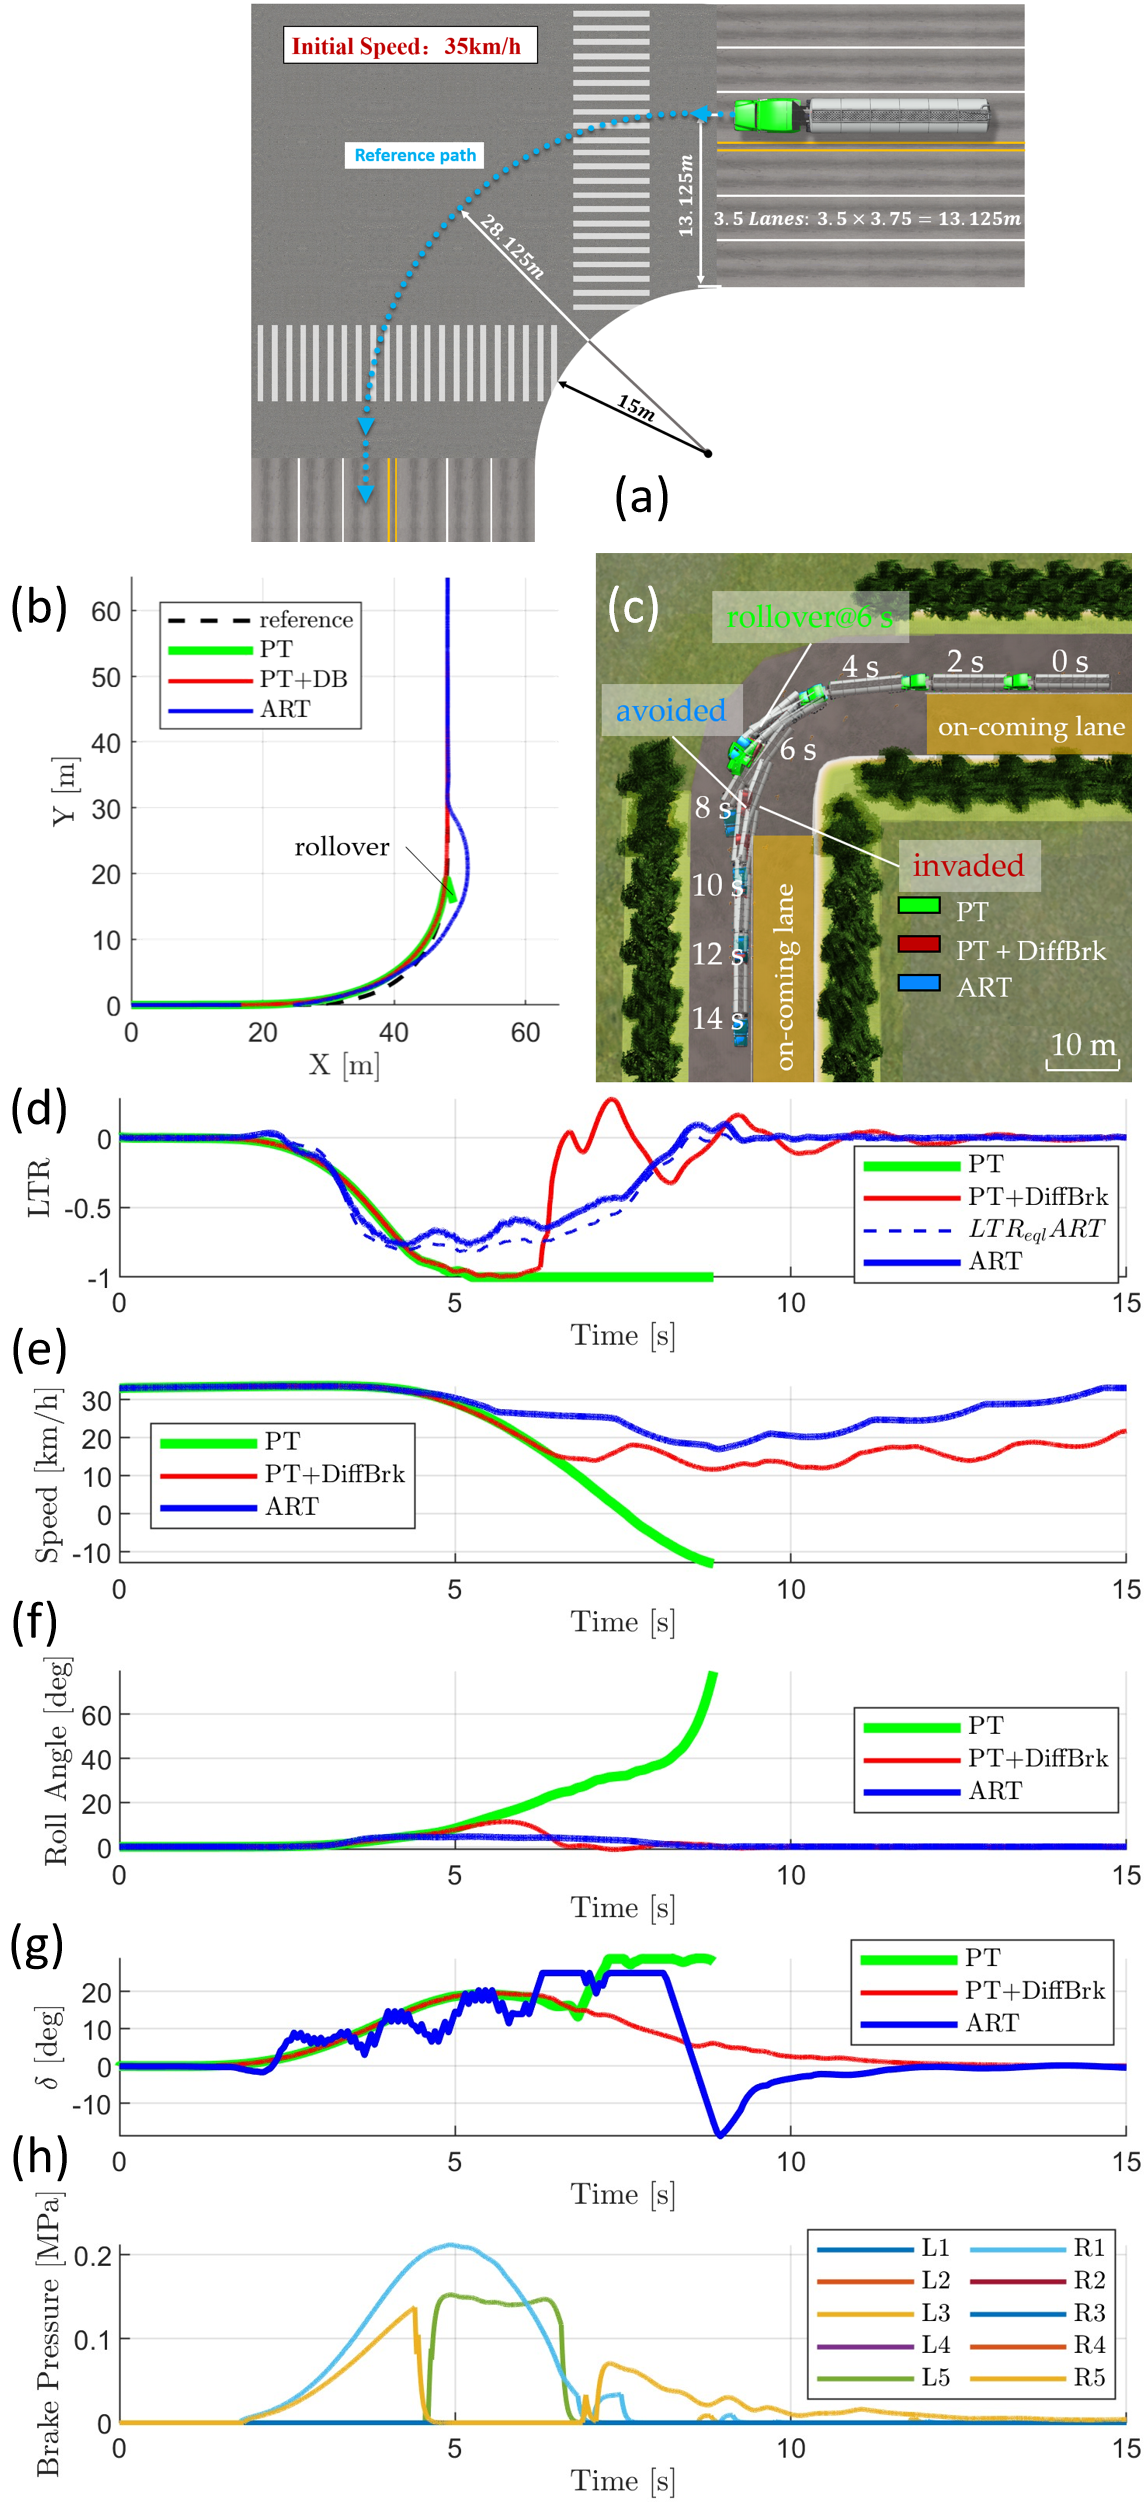
\includegraphics[width=3.3in]{fig/corner_results.png}
    \vspace{-0.3cm}
  \caption{left turning scenario simulation results. PT: preview tracking, DiffBrk: differential braking, ART: anti-rollover tracking. (a)Situation illustration (b)Tracking performance. (c)Simulation snapshots. (d)Lateral load transfer rate. (e)Speed profiles. (f)Roll angles. (g)Steering angles. (h)Brake Pressure for DiffBrk group.}
  \label{fig:left_corner}
  \vspace{-0.5cm}
\end{figure}

According to regulations \cite{WJG203-2006}, minimum turning radii are required for left and right turns. For right turns, a curb radius of 10-20 m is needed when the design speed exceeds 20 km/h \cite{UrbanCrossDesign}. Due to the kinematic constraints of semi-trailers, they require larger turning radii \cite{CrossCornerRadius}. A 15 m right turning radius was chosen for the smooth turning of the semi-tanker truck. When making a left turn from the innermost lane to another innermost lane, the left turning radius is 28.125 m, equivalent to adding 3.5 lane widths to the base right turning radius, as shown in Fig. \ref{fig:left_corner}(a). In simulation, initial vehicle speed is set to 35 km/h, corresponding to the speed encountered at a green light before the left turn.

As shown in Fig. \ref{fig:left_corner}, the controller anticipates potential rollover through model predictive control and takes gentler steering actions to avoid it while making minor steering adjustments to counteract sloshing effects. The $LTR_{eql}$ is successfully controlled within the soft constraint of ±0.75, effectively preventing rollovers while allowing for minor deviations from the desired path within acceptable limits. In contrast, the preview tracking group, which only considers path tracking without accounting for vehicle dynamics and the influence of liquid, experiences a rollover during the 6th second of cornering. Although the path may be safe for regular vehicles, it can lead to rollovers for liquid tank trucks. With differential braking added, extra yaw moment and slowed-down speed contribute together to the safe result, while still not able to avoid $LTR$ to reach -1 for at least 1 second.

Two conclusions can be drawn. Firstly, the $LTR_{eql}$ calculated by the controller closely aligns with the LTR obtained from actual tire force calculations using TruckSim, indicating that $LTR_{eql}$ accurately reflects the vehicle's rollover dynamics and is suitable for anti-rollover control for autonomous driving. Secondly, as discussed in Section III-B, by imposing a soft constraint $|LTR_{eql}| < 0.75$ on the system output $LTR_{eql}$, the controller effectively enforces this constraint and plans proactive steering actions to achieve path tracking while suppressing sloshing and preventing rollovers. 


\subsubsection{High-speed Single lane change scenario}


\begin{figure}[!bt]
  \centering
    \vspace{-0.3cm}
    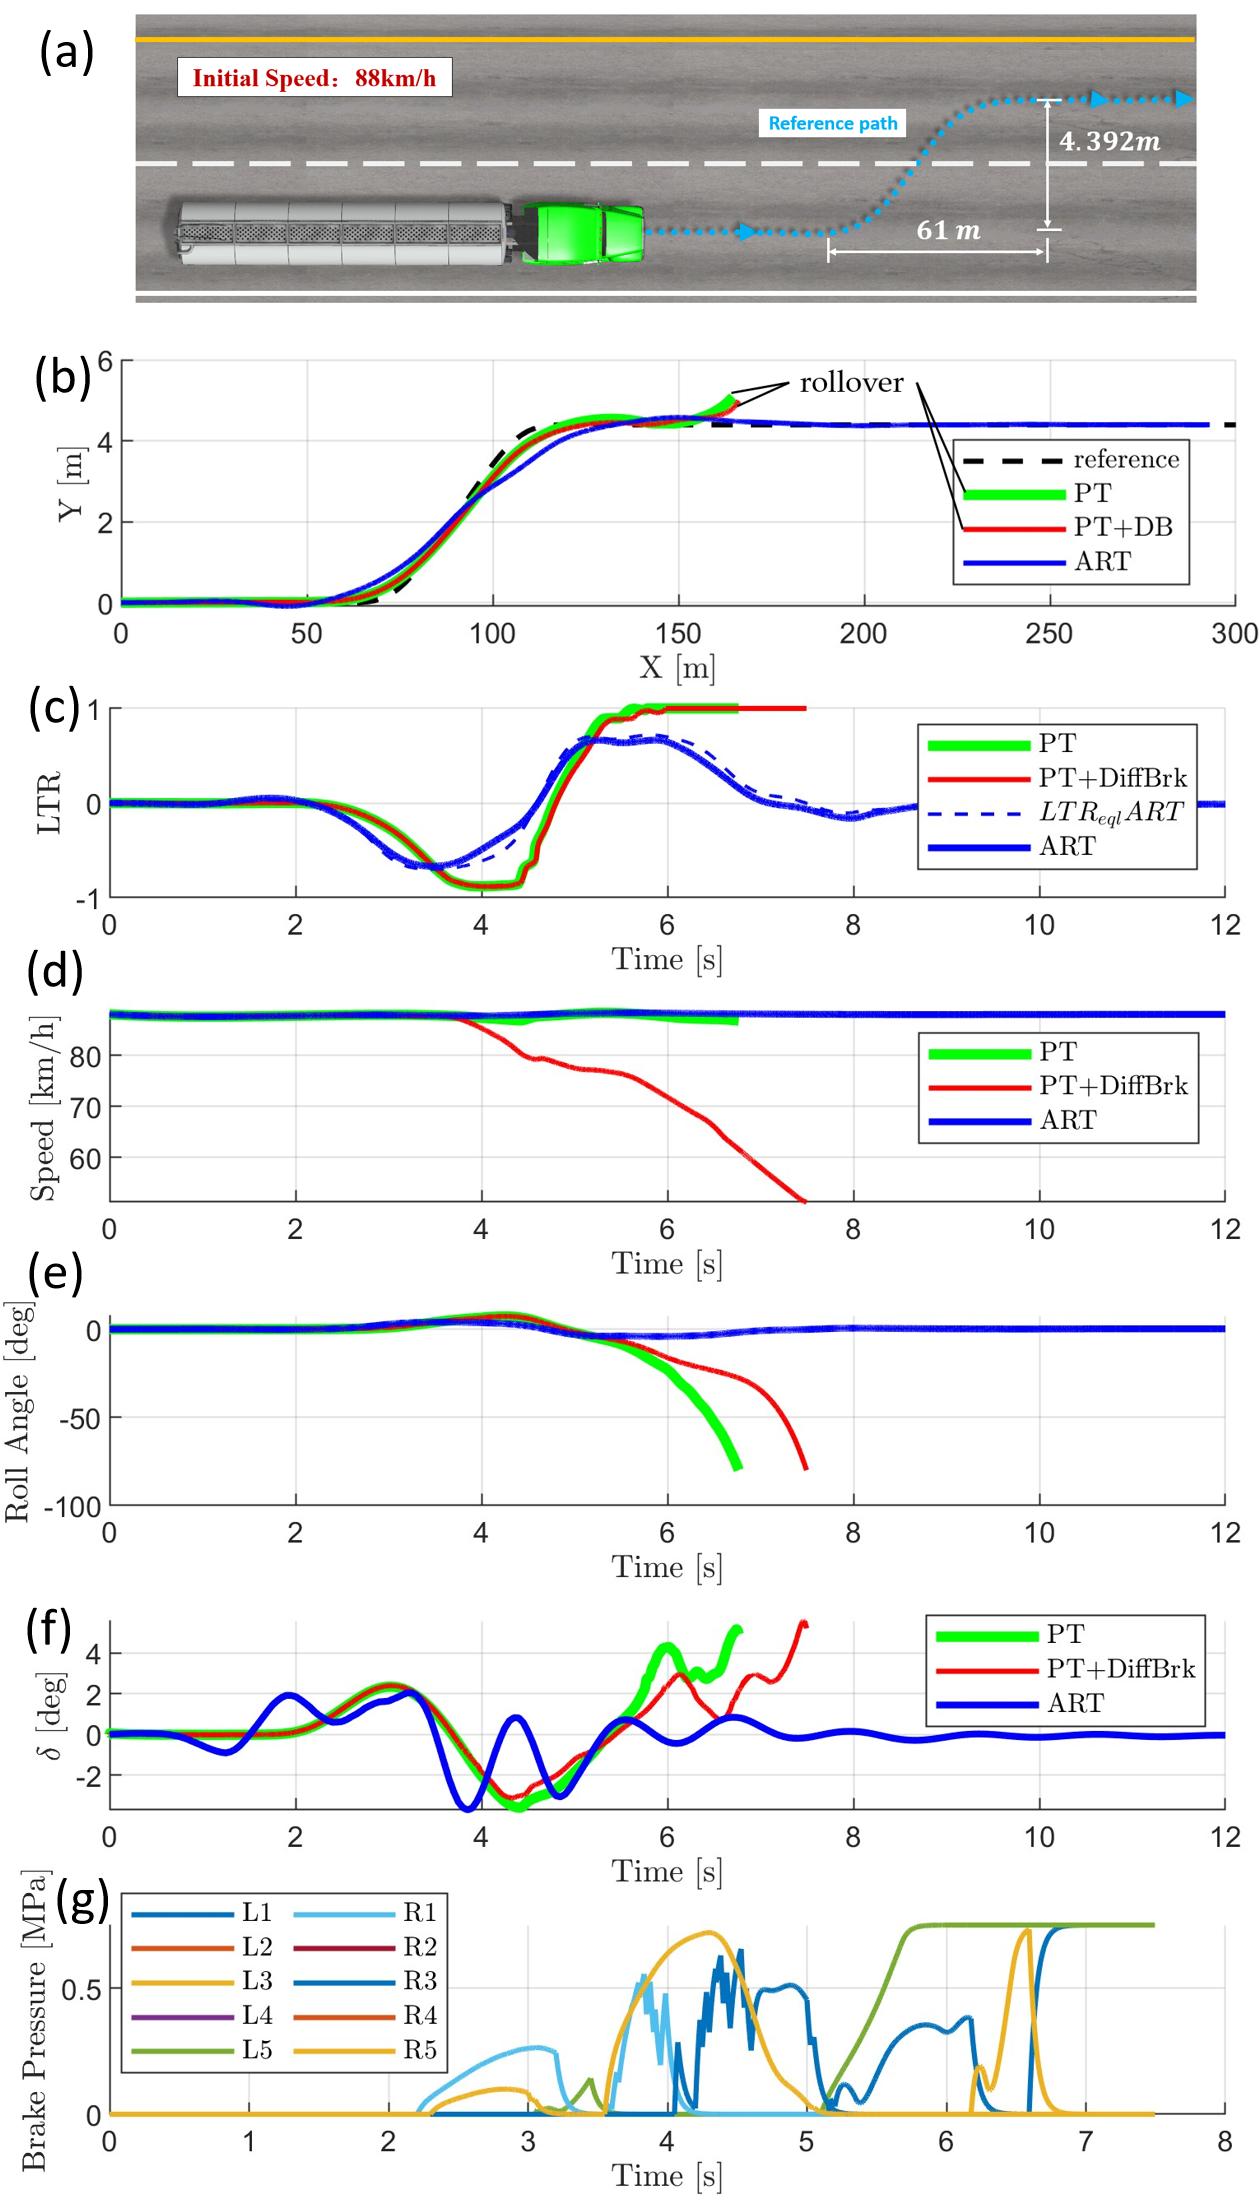
\includegraphics[width=3.3in]{fig/slc_results.png}
    \vspace{-0.3cm}
  \caption{High-speed single lane change scenario simulation results. PT: preview tracking, DiffBrk: differential braking, ART: anti-rollover tracking. (a)Situation illustration (b)Tracking performance. (c)Lateral load transfer rate. (d)Speed profiles. (e)Roll angles. (f)Steering angles. (g)Brake Pressure for DiffBrk group.}
  \label{fig:SLC}
  \vspace{-0.6cm}
    \end{figure}
For the high-speed single lane change scenario, it is set according to standard SAE-J2179, as shown in Fig. \ref{fig:SLC}(a). The initial speed is 88 $km/h$, and the shift to the left lane with a width of 4.392 $m$ within 61 $m$. A third-order Hermite interpolation method is used to interpolate key points, ensuring a smooth variation of the reference path curvature.

Fig. \ref{fig:SLC} shows that to prevent rollovers, the anti-rollover group starts making slight steering adjustments before the lane change at 50 $m$. However, due to extreme conditions and the soft constraint imposed on the MPC controller ($|LTR_{eql}| < 0.75$), tracking performance is sacrificed to guarantee rollover prevention. In contrast, the preview tracking group experiences a rollover after the lane change in the 6th second. Even with differential braking and the speed lowered to around 50 km/h, rollover is still not able to be avoided. Despite sacrificing some tracking performance, the anti-rollover group maintains an acceptable tracking error but keeps $LTR$ in a safe range.

\subsubsection{Short Distance Double lane change scenario}


\begin{figure}[!bt]
  \centering
    \vspace{-0.3cm}
    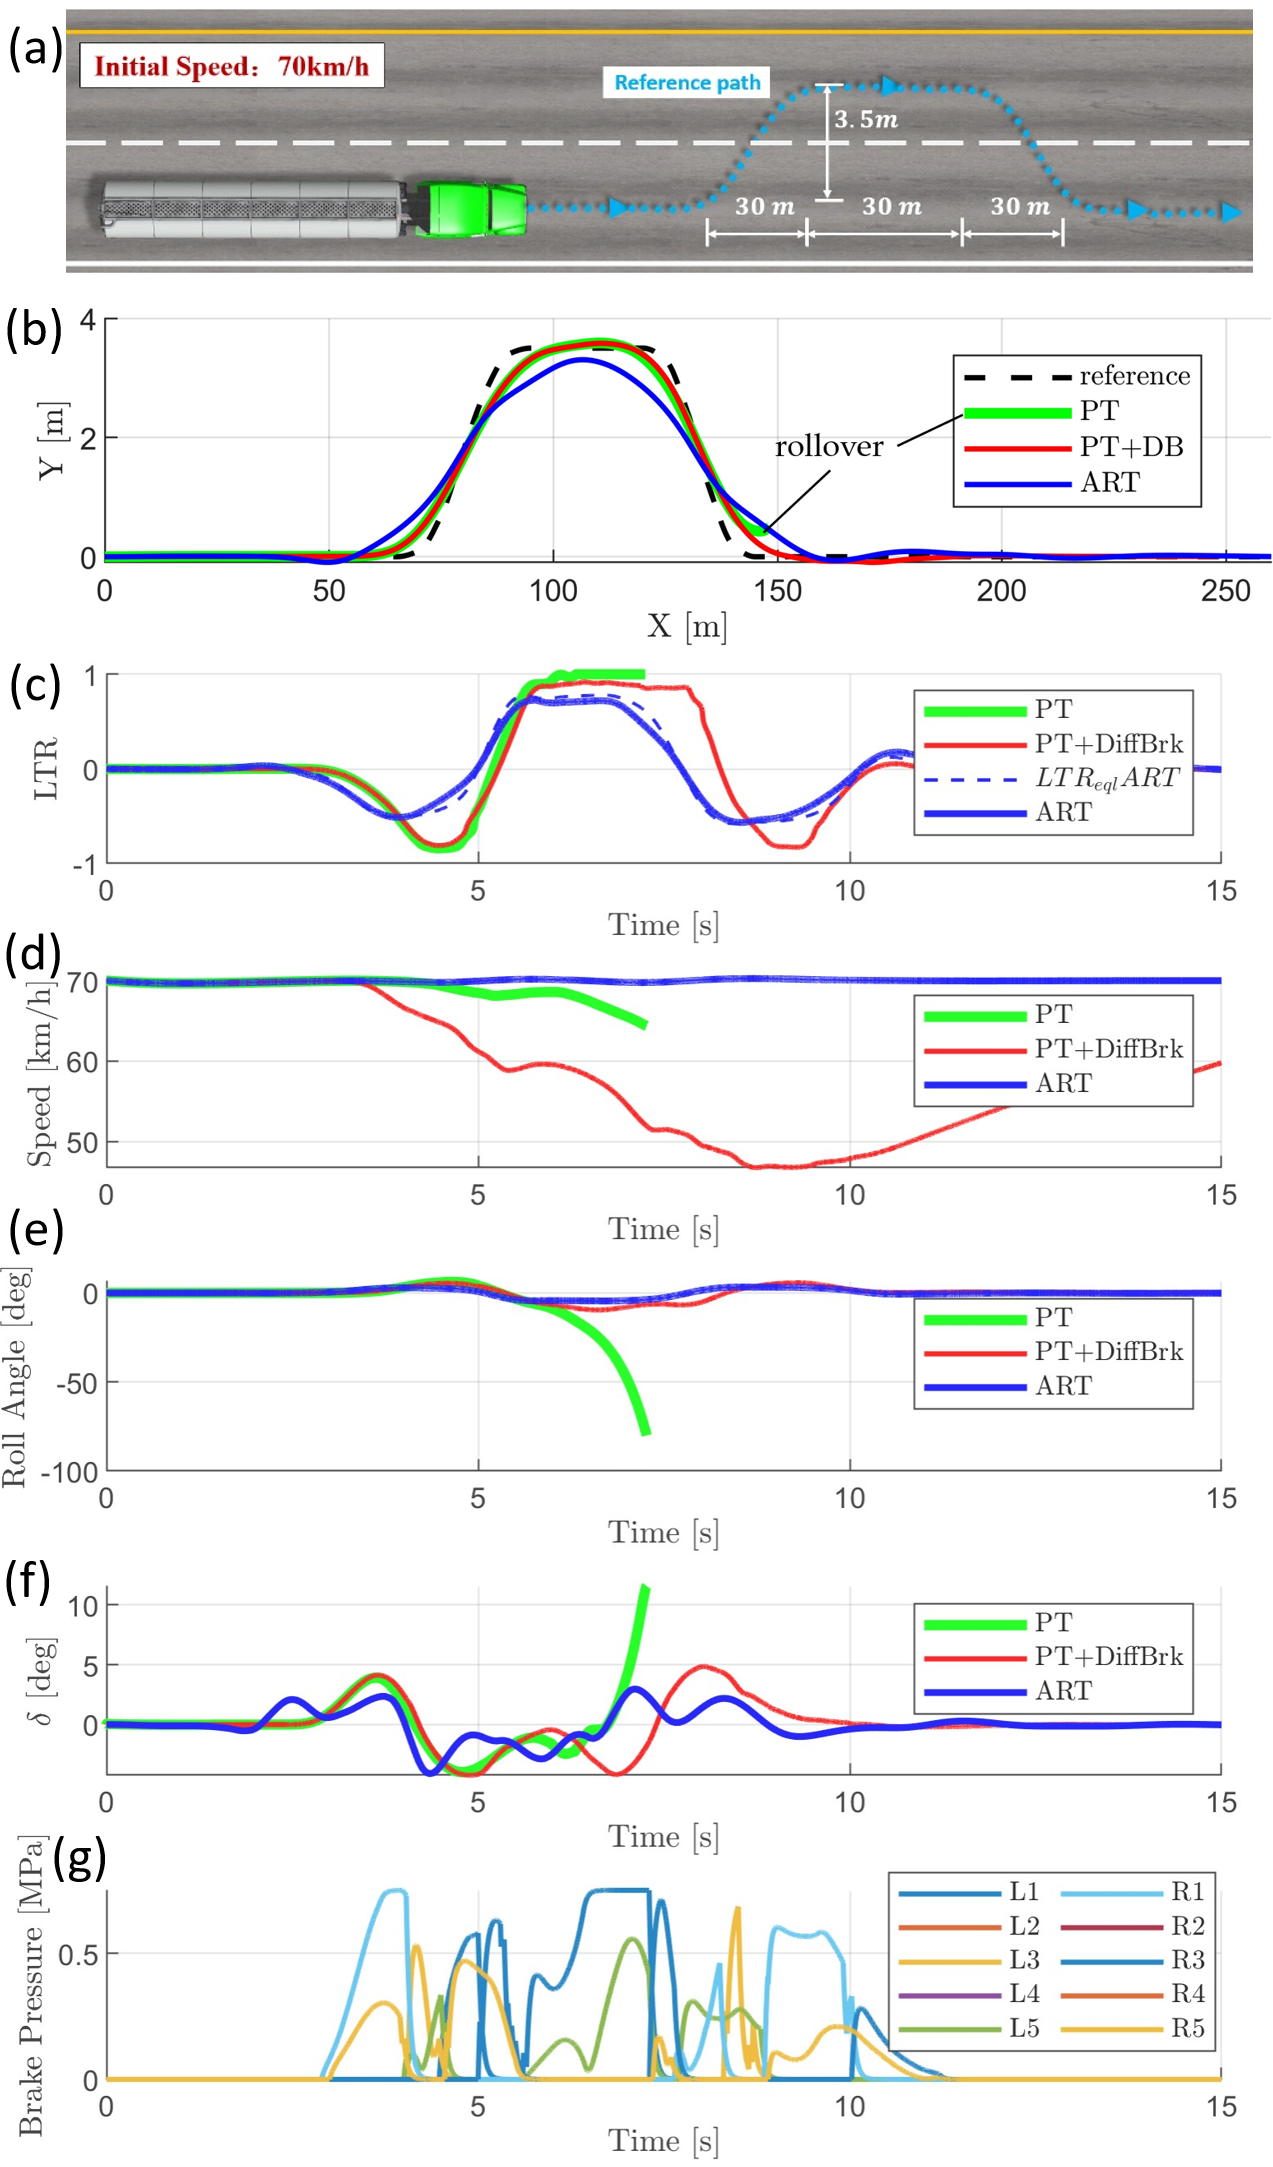
\includegraphics[width=3.3in]{fig/dlc_results.png}
    \vspace{-0.3cm}
  \caption{Short distance double lane change scenario simulation results. PT: preview tracking, DiffBrk: differential braking, ART: anti-rollover tracking. (a)Situation illustration (b)Tracking performance. (c)Lateral load transfer rate. (d)Speed profiles. (e)Roll angles. (f)Steering angles. (g)Brake Pressure for DiffBrk group.}
  \label{fig:DLC}
  \vspace{-0.6cm}
\end{figure}

Fig. \ref{fig:DLC} shows the validation of control effectiveness in a short-distance double lane change scenario. This scenario involves changing lanes laterally by 3.5 m within a distance of 30 m at a speed of 70 km/h, followed by straight-line driving for another 30 m, and then changing back within 30 m. Simulation results revealed that the preview tracking group experienced a rollover at a speed of 62 km/h, indicating the high risk involved at the experimental speed of 70 km/h. In contrast, the anti-rollover group started steering earlier at 60 m, made smaller lane changes, and kept $LTR_{eql}$ within the soft constraint to prevent rollover under extreme conditions, as shown in Fig. \ref{fig:DLC}. In contrast, with differential braking, even if rollover is avoided, $LTR$ saturated for at least 2.5 s, and the speed is much lowered causing longitudinal sloshing which introduces new problems.

\subsection{Analysis of Simulation Results}

From the simulation results of the three typical extreme conditions, the following conclusions can be drawn:

\begin{itemize}
    \item Paths that can be followed by regular vehicles may lead to rollovers for partially loaded tank trucks.
    \item $LTR_{eql}$, the equivalent value from suspension forces, aligns well with the actual LTR and effectively reflects the vehicle's rollover dynamics.
    \item By imposing soft constraints on the output variables, the controller can effectively prevent rollovers of tank trucks while maintaining approximate linear sloshing of the liquid and acceptable tracking performance.
    \item Differential braking is effective in preventing rollover, but has limited ability in enhancing rollover resistance while sacrificing too much speed, introducing more problems to be solved.
\end{itemize}


